 
%%%%%%%%%%%%%%%%%%%%%%%%%%%%%%%%%%%%%%%%%%%%%

\section[TS Cell Model]{T~Stellate Cell Model: Optimisation of Three Chopper Subtypes}

\subsection{Background}
 
Accurate modelling of the cochlear nucleus, in particular chopper units and T~stellate cells.
\yellownote{Expand background}

This work expands on the extracellular classification by \citep{BlackburnSachs:1989} into slowly or transiently adapting and sustained choppers in cats.


Figure~\ref{fig:PaoliniAIV} shows the intracellular acoustic classification of chopper units in the rat into three distinct types \citep{PaoliniClareyEtAl:2005}: CS chopper sustained, and two transient choppers, CT1 and CT2.

The work by Tony Paolini, Janine Clarey, Karina Needham and others at the Royal Victorian Eye and Ear Hospital were pivotal in collecting the T stellate cell experimental data used in this section.

The intracellular traces in Figure~\ref{fig:PaoliniAIV} will form the basis for the optimisation routine of T~stellate cell model along with the CV statistics of each chopper type.  

\begin{figure}[htb]
\centering%
\subfloat[Chopper Sustained]{\includegraphics[keepaspectratio,width=0.3\textwidth]{TStellate/CS-01-864-004-a}}\hfill%\quad%
\subfloat[Chopper Transient 1]{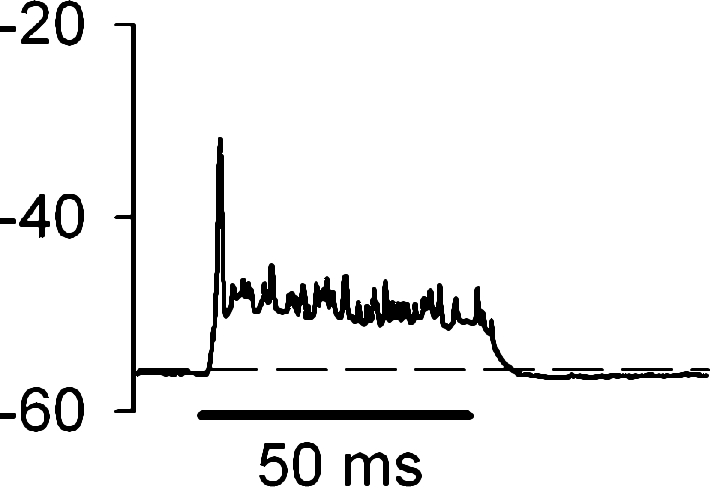
\includegraphics[keepaspectratio,width=0.3\textwidth]{TStellate/CT1-01-857-007}}\hfill%\\
\subfloat[Chopper Transient 2]{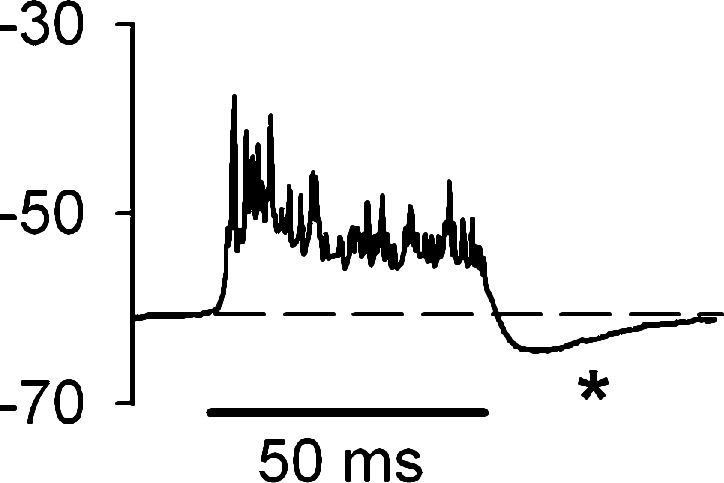
\includegraphics[keepaspectratio,width=0.3\textwidth]{TStellate/CT2-01-305-014}}%\quad%
%\subfloat[Onset Chopper]{\resizebox{0.35\textwidth}{!}{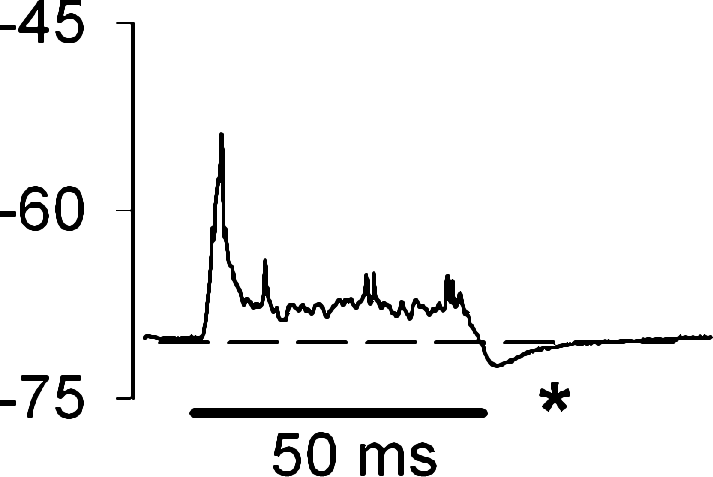
\includegraphics{TStellate/OC-99-812-013}}}
\caption[Average intracellular response data in stellate cells in rats.]{Average intracellular response to CF tone 30dB above depolarisation threshold in stellate  cells~\citep[Reproduced from Fig.~2, ][]{PaoliniClareyEtAl:2005}.
A. Sustained chopper unit 01-864-004, CF 3.8~kHz,
B. Transient chopper type 1 unit 01-857-007, CF 8.9~kHz.
C. Transient chopper type 2 unit 01-305-014 CF 12.3~kHz.
%D. Onset chopper unit  99-812-013.
Hyper polarisation after tone indicated by asterisk.  \label{fig:PaoliniAIV}}
\end{figure}
\yellownote{Permission needed for Paolini plots}

The categorisation via coefficient of variation is shown in Figure~\ref{fig:PaoliniCVdata}.
Sustained choppers maintain a stable CV below 0.2 throughout the entire stimulus. The transient chopper optimisation had two types defined by \citep{PaoliniClareyEtAl:2005}.
The first CT type is categorised with CV starting below 0.2 then rising, hence the name transient, but stays below 0.3.
The second CT type is regular in the first 10 ms period, but rises to 0.3 or above throughout the stimulus.

\begin{figure}[htb]
\centering%
%\resizebox{0.6\textwidth}{!}{
\includegraphics{TStellate/PaoliniCV.eps}
%}
\caption{Regularity in chopper units \citep[Data reproduced from Fig.~2,~][]{PaoliniClareyEtAl:2005}}
\label{fig:PaoliniCVdata}
\end{figure}


\subsection{Implementation}

\yellownote{Para 1: Nordlie table~\ref{tab:TSModelSummary}A. Using R\&M  type I-t, Other previous models}
\yellownote{Synaptic inputs known and unknown, included and not included in model.  Previous work include and excludes}

Figure~\ref{fig:TSinputs} shows the expected response of a T~stellate cell to individual connections from different cells in the CN stellate network.
The membrane parameters for the single compartment T~stellate cell model are default except for sodium conductance set to zero.
In this example, excitation from the afferent \ANF~inputs (\LSR~Figure~\ref{fig:TSinputs}A and \HSR~Figure~\ref{fig:TSinputs}B) show a large depolarisation.
\HSR~inputs show a rapid onset and a slowly adapting sustained depolarisation.


\yellownote{Actual parameters: diameter =19.5$\mu$m, $\gNa=0$, $\gKHT=0.0189416$ S cm$^{-2}$, $\gleak=0.000473539$ S cm$^{-2}$, $\gh=$6.20392e-05 S cm$^{-2}$, $\gKA=0.01539$ S cm$^{-2}$, $\Eleak=-65$ mV, $\ENa=50$ mV, $\EK=-70$ mV.}


\begin{figure}[htb]
\centering%
\includegraphics[keepaspectratio,width=0.9\textwidth]{TStellate/baseline_exc}\\
\includegraphics[keepaspectratio,width=0.9\textwidth]{TStellate/baseline_inh}
\caption[Response of T~stellate cells to isolated synaptic inputs]%
{Intracellular membrane voltage response of a T~stellate cell model to isolated synaptic inputs.
A pure tone stimulus of 8.2~kHz at 85 dB~SPL was presented to the CN network. The CF of the recorded TS unit was 8.267~kHz.
Single stimulus responses are shown as a thin line and average response over 25 repetitions is shown as the dark line.
A. 30 LSR ANF synapses.
B. 20 HSR ANF synapses.
C. 20 D stellate cell glycinergic synapses.
D. 15 Golgi cell \GABAa synapses.
All weights were set to $0.0005\,\mu{\rm S}$ and the sodium conductance (\gNa)set to zero.
The parameters for synapse's were: excitatory (tau = 0.36 ms), glycinergic (tau1=0.4 and tau2=2.5 ms), and GABAergic (tau1=0.26 and tau2=5.43 ms).\label{fig:TSinputs}}
\end{figure}

\begin{figure}[htb]
\centering%
% \resizebox{0.9\textwidth}{!}{\includegraphics{TStellate/baseline_jitter}}
\includegraphics[keepaspectratio=true,width=0.9\textwidth]{TStellate/baseline_jitter}
  % \caption[Response of T~stellate cells to isolated synaptic
  % inputs]{Intracellular membrane voltage response of a T~stellate cell
  %   model to isolated synaptic inputs. A pure tone stimulus of 8.2~kHz at
  %   85 dB~SPL was presented to the CN network. The CF of the recorded
  %   T~stellate cell was 8.267~kHz.  Single stimulus responses are shown as
  %   a thin line and average response over 25 repetitions is shown as the
  %   dark line. A. 30 LSR ANF synapses. B. 20 HSR ANF synapsexs. C. 20 D
  %   stellate cell glycinergic synapses. D. 15 Golgi cell GABA$_{\rm A}$
  %   synapses. All weights were set to $0.0005\,\mu{\rm S}$ and the sodium
  %   conductance set to zero.  The parameters for synapases were: excitatory
  %   (tau = 0.36 ms), glycinergic (tau1=0.4 and tau2=2.5 ms), and
  %   GABAergic (tau1=0.26 and tau2=5.43 ms).\label{fig:TSExcinputs}}
\caption[]{Jitter of AN input T~stellate Optimisation results}\label{fig:CSjitter}
\end{figure}





%%% Local Variables:
%%% mode: latex
%%% mode: tex-fold
%%% mode: visual-line
%%% TeX-master: "SimpleResponses"
%%% TeX-PDF-mode: nil
%%% End:
